\subsection{Results}

\begin{frame}{Evaluation Methodology}
    \begin{itemize}
        \item \textbf{Dataset}: Validation set from the before-mentioned dataset
        \item \textbf{Degradation}: Motion blur with varying kernel sizes
        \item \textbf{Methods Compared}:
        \begin{itemize}
            \item DPS (Diffusion Posterior Sampling)
            \item RED-Diff (Regularization by Denoising)
        \end{itemize}
        \item \textbf{Evaluation Metrics}:
        \begin{itemize}
            \item PSNR (Peak Signal-to-Noise Ratio) in dB
            \item SSIM (Structural Similarity Index)
        \end{itemize}
    \end{itemize}
\end{frame}

\begin{frame}{Metric Computation Process}
    \begin{itemize}
        \item \textbf{For each test image}:
              \begin{enumerate}
                  \item Load ground truth image $x_{gt}$
                  \item Apply motion blur: $y = K(x_{gt})$
                  \item Reconstruct using DPS: $x_{dps} = \text{DPS}(y, K)$
                  \item Reconstruct using RED-Diff: $x_{red} = \text{RED-Diff}(y, K)$
                  \item Compute metrics: $\text{PSNR}(x_{gt}, x_{rec})$, and $\text{SSIM}(x_{gt}, x_{rec})$
              \end{enumerate}
    \end{itemize}
\end{frame}

\begin{frame}{PSNR}
    Figure \ref{fig:psnr_results} shows the PSNR values for both methods across different kernel sizes.
    \begin{figure}
        \centering
        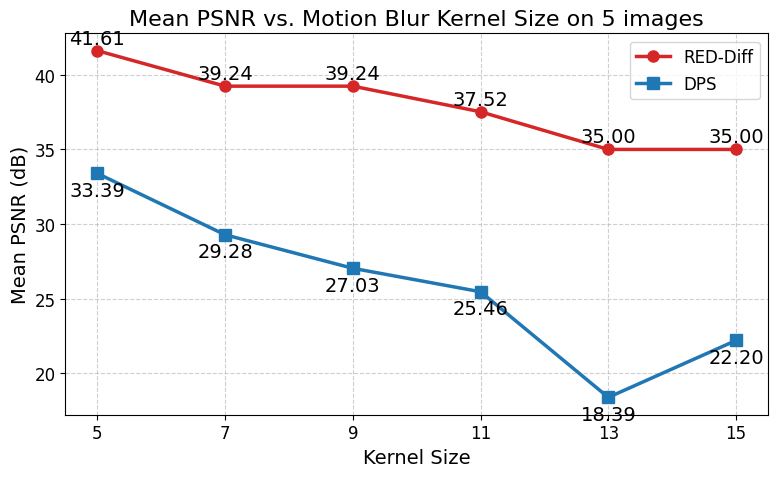
\includegraphics[width=0.5\textwidth]{media/mean_psnr_over_kernels.png}
        \caption{PSNR values for DPS and RED-Diff across different kernel sizes.}
        \label{fig:psnr_results}
    \end{figure}
\end{frame}

\begin{frame}{SSIM}
    Figure \ref{fig:ssim_results} illustrates the SSIM values for both methods across different kernel sizes.
    \begin{figure}
        \centering
        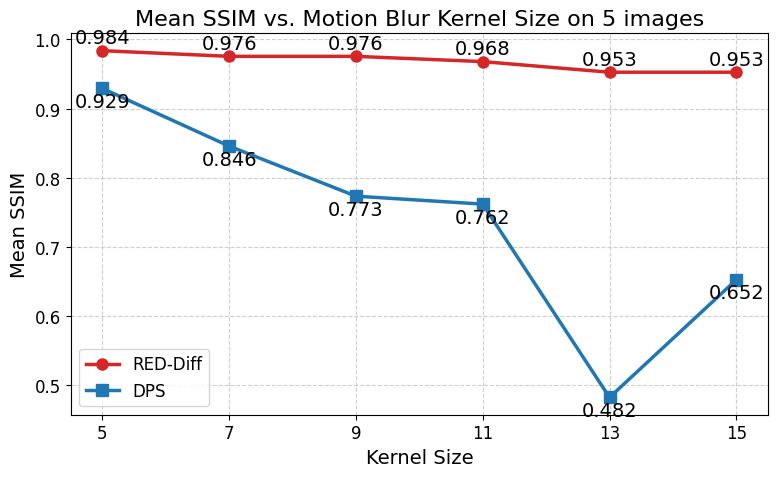
\includegraphics[width=0.5\textwidth]{media/mean_ssim_over_kernels.png}
        \caption{SSIM values for DPS and RED-Diff across different kernel sizes.}
        \label{fig:ssim_results}
    \end{figure}
\end{frame}

% \begin{frame}{Performance Analysis}
%     \begin{itemize}
%         \item \textbf{Trend Analysis}:
%               \begin{itemize}
%                   \item Both methods show performance degradation with larger kernels, even though the RED-Diff method generally outperforms DPS.
%                   \item PSNR and SSIM correlate with blur severity
%               \end{itemize}
%     \end{itemize}
% \end{frame}

\begin{frame}{Results - Qualitative Analysis}
\begin{itemize}
    \item \textbf{Qualitative Assessment}:
          \begin{itemize}
              \item Side-by-side comparisons: Original → Blurred → Reconstructed
              \item Visual quality correlation with quantitative metrics
              \item Edge preservation and artifact analysis
          \end{itemize}
    \item \textbf{Key Findings}:
          \begin{itemize}
              \item RED-Diff better preserves fine details
              \item RED-Diff shows less artifacts compared to DPS
              \item RED-Diff keeps consistent performances across different kernel sizes
              \item DPS is more sensitive to kernel size variations, as shown in the PSNR and SSIM results
          \end{itemize}

    \item \textbf{Visual Results}: To better understand the performance of both methods, we will show visual results for both DPS and RED-Diff a visual comparison had been conducted and reported on kernel size equal to 7 in the next slides.
\end{itemize}
\end{frame}

\begin{frame}{Visual Results Summary - DPS}
    Figure \ref{fig:visual_results_dps} presents visual comparisons of the original, blurred, and reconstructed images for both methods for kernel size 7 using DPS.
    \begin{figure}
        \centering
        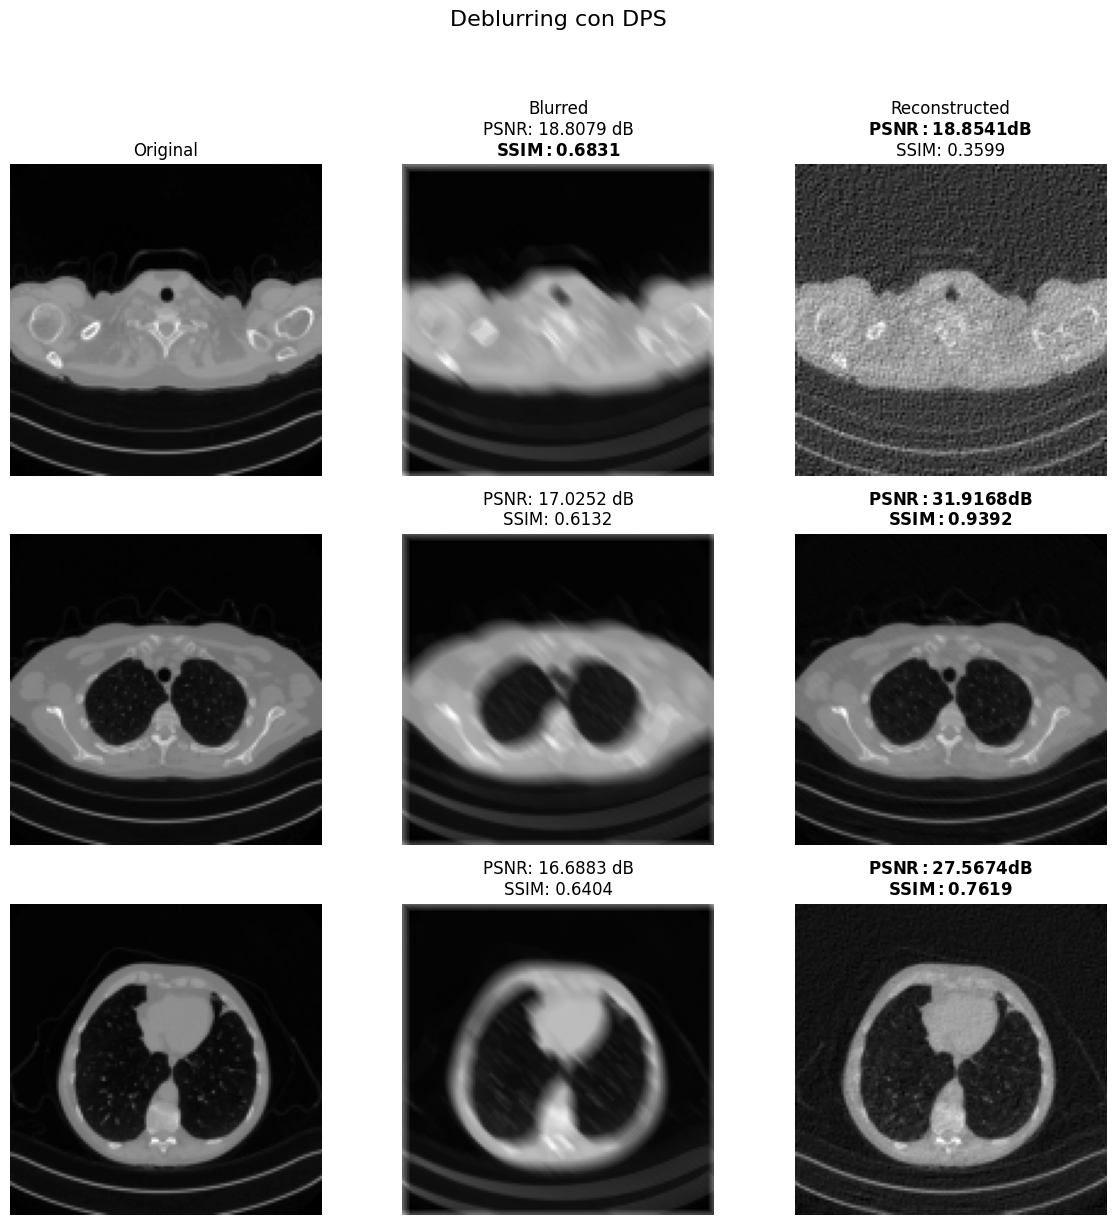
\includegraphics[width=0.5\textwidth]{media/deblurring_dps.png}
        \caption{Visual results for DPS.}
        \label{fig:visual_results_dps}
    \end{figure}

\end{frame}
\begin{frame}{Visual Results Summary - RED-Diff}
    Figure \ref{fig:visual_results_red_diff} presents visual comparisons of the original, blurred, and reconstructed images for both methods for kernel size 7 using RED-Diff.
    \begin{figure}
        \centering
        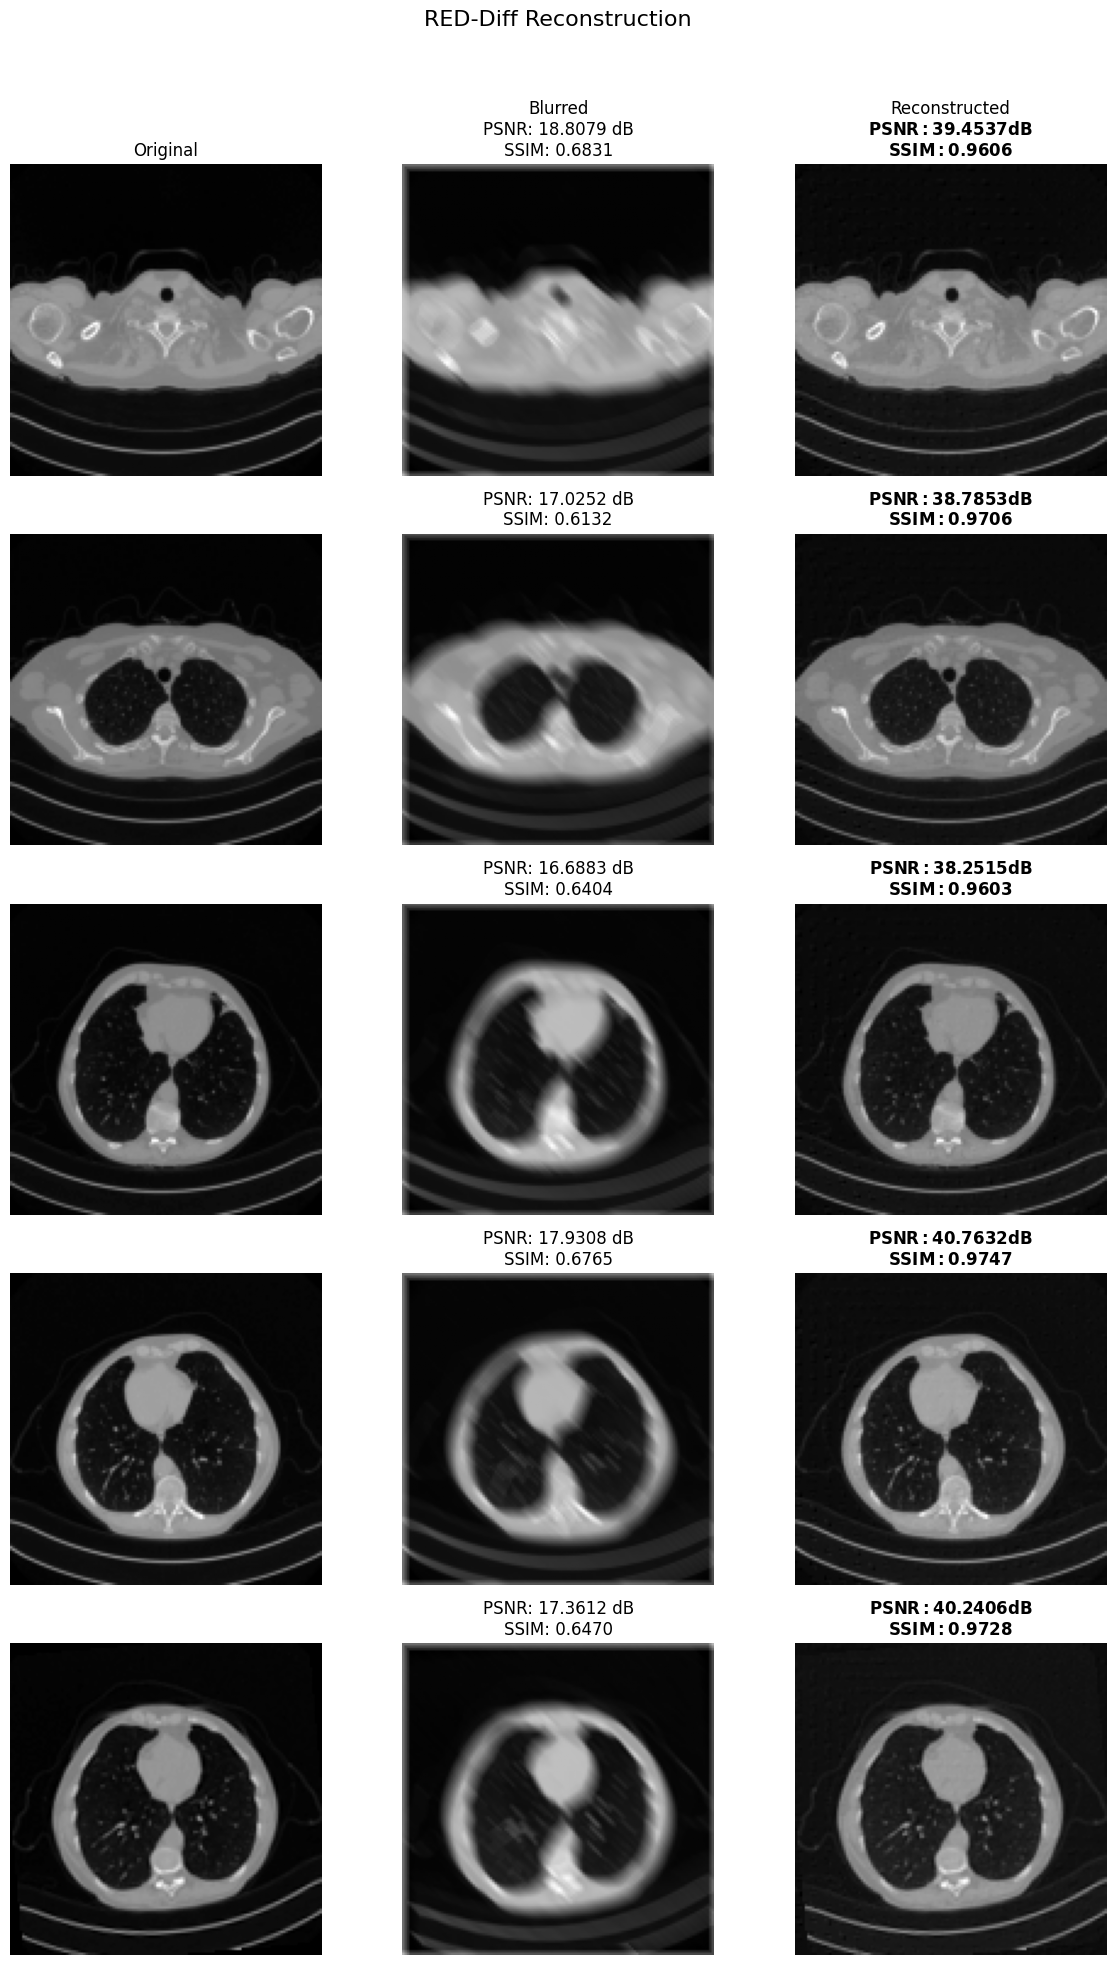
\includegraphics[width=0.5\textwidth]{media/deblurring_reddiff.png}
        \caption{Visual results for RED-Diff.}
        \label{fig:visual_results_red_diff}
    \end{figure}
\end{frame}

\begin{frame}{Scaling to 256x256}
    \begin{itemize}
        \item We explored training at a larger target size of $256\times256$ pixels.
        \item Due to hardware and Colab limits, full $256\times256$ training proved very slow.
        \item We expect comparable results at $256\times256$ because:
            \begin{itemize}
                \item Model architecture and training pipeline remain the same.
            \end{itemize}
        \item If $256\times256$ runs underperform, we can still approach $128\times128$-level results by:
            \begin{itemize}
                \item Leveraging our robust data augmentation to enrich the larger-scale inputs.
            \end{itemize}
        \item The implementation is flexible, so once faster hardware or longer runtimes are available, we can re-run full $256\times256$ experiments with minimal changes.
    \end{itemize}
\end{frame}
